\indent\indent The visualisation tool is automatically opened after a correlation process. It is also accessible on the start-up widget by clicking on the \textit{Open Analysis} button.\\
\newline
There is two type of element in the visualisation window:
\begin{itemize}
  \item A certain amount of plots
  \item A control area with information
\end{itemize}
\newline
The control area is fixed and displays information on the analysis and the current image selected.\\
You can navigate through the data using the two cursor available in the control area.\\

\begin{figure}[!h]
   \centering
   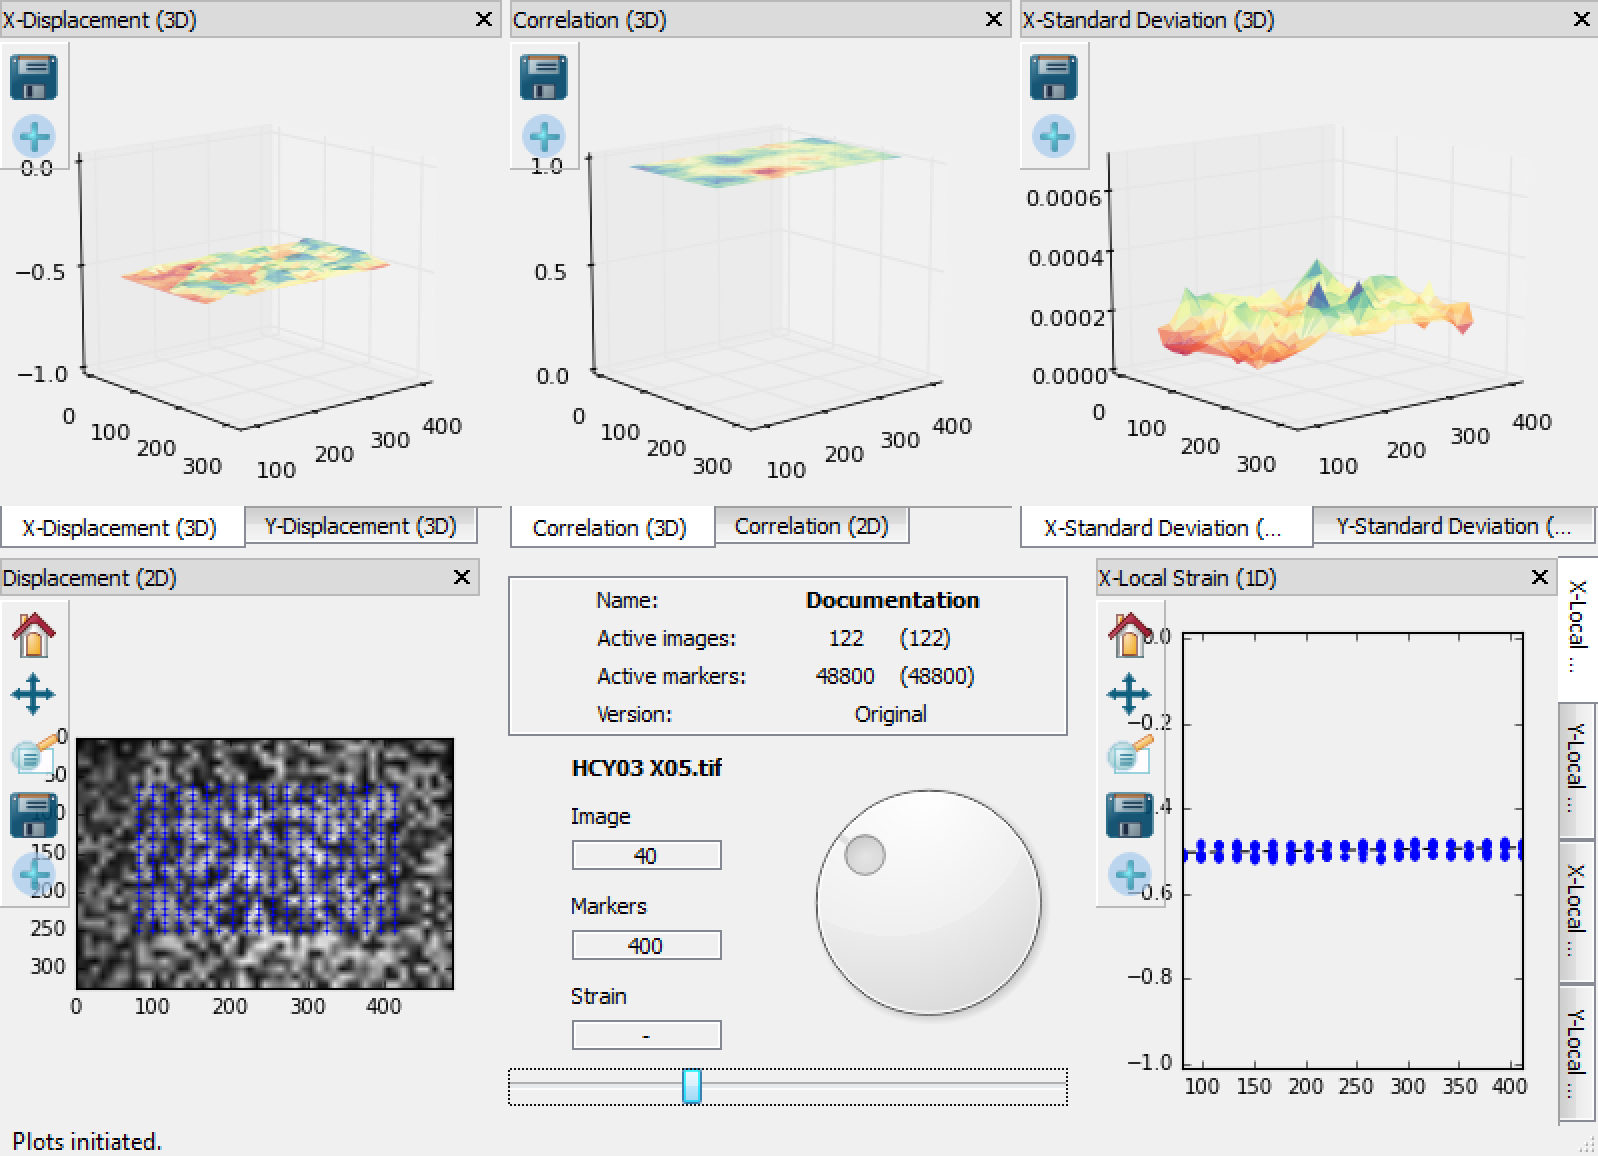
\includegraphics[scale=.4]{visualisation}
   \caption{Visualisation : Navigation through results}
\end{figure}

\newline
\noindent Plots are located around the control area and can be re-organized by the user.
\begin{itemize}
  \item Click and drag a plot to move it
  \item Close unwanted plots using the individual cross
  \item Open plots by right-clicking on an empty area or next to the menu
\end{itemize}
\newline
When the data is refreshed, only the visible opened plots are taken in account. For large analysis, closing unnecessary plots will sensibly decrease the refreshing time.\\
You can also stack plots on top of each other for a quick access. This will not affect the refreshing time as only visible plots are reloaded.\\
\newline
For each single plot, you can use the toolbar to save the plot as an image and zoom/pan on your data. Different display options are also available, click on the \textit{+} button in the toolbar to get access to parameters.
\vspace{.5cm}
\begin{figure}[!h]
   \centering
   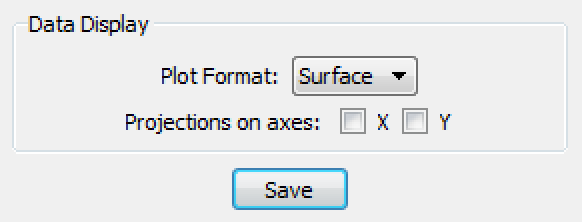
\includegraphics[scale=.8]{plot_options}
   \caption{Visualisation : 3D plots options}
\end{figure}
